\chapter{Forced Vibrations \& Resonance}


	In this chapter, we consider the effects of a \textbf{driving force} $F(t)$ on a system, where:
	\[ {F(t) = F_0 \cos(\omega t)} \]
	\begin{itemize}
		\item $\omega$ represents the \textbf{driving frequency}
		\item $\omega_0$ represents the \textbf{natural frequency} of the system, associated with a \textbf{free vibration} (see Chapter~\ref{ch:free-vibrations})
	\end{itemize}



We will see that...
\begin{itemize}
	\item As $\omega \to \omega_0$, the amplitude of oscillation increases
	\item ... whereas as $\omega$ gets farther away from $\omega_0$, the amplitude becomes smaller
	\item This phenomenon is known as \textbf{resonance}.
\end{itemize}

The system will initially have the tendency to vibrate at $\omega_0$, but it will eventiually vibrate at $\omega$. We thus have two stages:
\begin{enumerate}
	\item \textbf{Transient state}: we have a superposition of oscillations at frequencies $\omega$ and $\omega_0$. The free vibration gradually gets damped away until...
	\item \textbf{Steady state}: only the the driving vibration remains, so the system oscillates at $\omega$
\end{enumerate}

\section{Forced Oscillations without Damping: Steady State}
We will consider the \emph{steady state} of a forced oscillation with \emph{negligible damping}, ignoring the fact that we need damping to get past the transient state.

Force equation:
\begin{align}
	m\ddot{x} &= -kx + F_0 \cos(\omega t)  \notag \\
	\Longrightarrow
	\mcol{m}\ddot{x} + \kcol{k}x &= F_0 \cos(\omega t)	\label{ch4:eq-no-b}
\end{align}

The behaviour of a driven pendulum is illustrated in Figure~\ref{ch4:fig-no-damping-pendula}. 

\begin{figure}
	\centering
	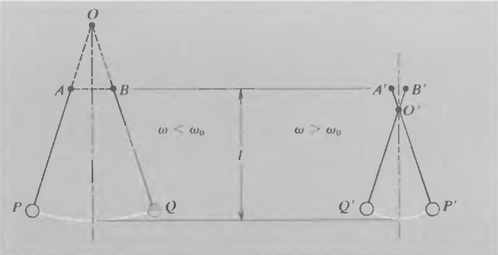
\includegraphics[scale=0.6]{phys232/Ch4-forced-no-damping-pendula.png} 
	\caption{The motion of simple pendula undergoing horizontal forced oscillations when (a) $\omega<\omega_0$ and (b) $\omega>\omega_0$.}\label{ch4:fig-no-damping-pendula}
\end{figure}

\begin{margintable}
	\normalsize
	\begin{tabular}{ccc}
		\hline
		Case & $A$ & {$\alpha$}  \\
		\hline
		$\omega < \omega_0$ & large & 0° \\
		$\omega > \omega_0$ & small & 180° \\
		\hline
	\end{tabular}
	\vspace{0.5em}
	\caption{Summary of cases~(a) and (b). Note that $\alpha$ represents the phase difference by which the driving force \emph{leads} the displacement.}
	\label{ch4:tbl-no-damping-results}
\end{margintable}

\paragraph{Case (a): $\omega < \omega_0$}
If the driving force's frequency is much lower than the natural frequency...
\begin{itemize}
	\item We expect a low acceleration (since $\ddot{x} \propto \omega^2$).
	\item So, the $\kcol{k}x$ term dominates over $\mcol{m}\ddot{x}$; i.e. the response is controlled by the \kcol{stiffness} of the string.
	\item The phase delay between the driving force and the displacement is $\alpha=0$.
	\item Thus, the amplitiude will be $A\approx F_0/k$%
		\footnote{At $x=A$, we have $F_0 \approx kA$, so $A\approx F_0/k$.}
\end{itemize}


\paragraph{Case (b): $\omega > \omega_0$}
If the driving force's frequency is much higher than the natural frequency...
\begin{itemize}
	\item We expect a higher acceleration (since $\ddot{x} \propto \omega^2$).
	\item So, the $\mcol{m}\ddot{x}$ term dominates over $\kcol{k}x$; i.e. the response is controlled by the \mcol{inertia} of the string.
	\item We expect a relatively small $A$, opposite in phase with the driving force -- i.e. the driving force leads the displacement by a phase difference of $\alpha=180$.%
	\footnote{Notice that in Figure~\ref{ch4:fig-no-damping-pendula}b, when $F$ is to the left, $x$ is to the right; when $F$ is to the right, $x$ is to the left.}
\end{itemize}

The observations in cases (a) and (b) are summarized in Table~\ref{ch4:tbl-no-damping-results}.



\subsection{Responant response ($\omega = \omega_0$)}

We will now examine why we obtain a much higher amplitude (the \textbf{resonant amplitude}) when $\omega = \omega_0$.

Assume we are in the steady state; i.e. the natural oscillations are not present. Hence:
\begin{align}
	x &= C\cos(\omega t) \notag \\
	\Longrightarrow
	\ddot{x} &= -\omega^2 C\cos(\omega t)	\label{ch4:eq-acc-forced-no-b}
\end{align}

Substitute \eqref{ch4:eq-acc-forced-no-b} into \eqref{ch4:eq-no-b}:
\begin{align*}
	-m\omega^2 C\cancel{\cos(\omega t)} + kC\cancel{\cos(\omega t)} &= F_0\cancel {\cos(\omega t)} \\
	C(k-m\omega^2) &= F_0
\end{align*}
\begin{equation*}
	 C = \frac{F_0}{k-m\omega^2} = \frac{F_0/m}{\omega_0^2-\omega^2} 
\end{equation*}

To avoid working with negative values of $C$, let $A=|C|$. Use $\alpha$ again to represent the phase difference by which the driving force leads $x$. Therefore:
\begin{equation}
\boxed{
	\begin{split}
		x &= A \cos(\omega t + \alpha)  \\
		\text{where }
		\alpha &= 
		\begin{cases}
			0 & \text{if } \omega<\omega_0 \\
			\pi & \text{if } \omega>\omega_0
		\end{cases}
		\\
		\text{and }
		A &= \left| \frac{F_0/m}{\omega_0^2-\omega^2}  \right| 
	\end{split}
}
\label{ch4:eq-soln-no-b}
\end{equation}


\begin{marginfigure}
	\centering
	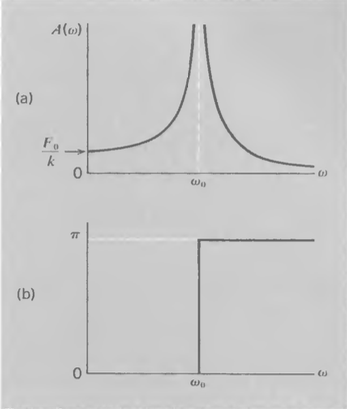
\includegraphics[scale=0.5]{phys232/Ch4-forced-no-damping-A.png} \caption{(a) Absolute amplitude of forced oscillations (no damping) as a function of $\omega$; (b) phase lag of $x$ with respect to the driving force, as a function of $\omega$.}	\label{ch4:fig-no-damping-A}
\end{marginfigure}

The results in \eqref{ch4:eq-soln-no-b} are plotted in Figure~\ref{ch4:fig-no-damping-A}. Notice that as $\omega\to\omega_0$, $C\to \infty$.


\subsection{Resonant response, using complex exponentials}
Recall \eqref{ch4:eq-no-b}:
\[ m\ddot{x} + kx = F_0 \cos(\omega t) \]

Visualize the driving force $F_0 \cos(\omega t)$ as the real component of $F_0 e^{j\omega t}$.
Assume $x=\Re(z)$, such that:
\[ m\ddot{z} + kz = F_0 e^{j\omega t}\]

Assume the following solution:
\[z = Ae^{j(\omega t+\alpha)} \]

Substitute in \eqref{ch4:eq-acc-forced-no-b}:
\begin{align*}
	(-m\omega^2 A + kA)e^{j(\cancel{\omega t} + \alpha)} &= F_0 \, \cancel{e^{j\omega t}} \\
	A(-\omega^2 + \omega_0^2)e^{j\alpha} &= \frac{F_0}{m} \\
	A(\omega_0^2 - \omega^2 ) &= \frac{F_0}{m} e^{-j\alpha} \\
	\Longrightarrow
	\underbrace{A(\omega_0^2 - \omega^2 )}_\text{real} &= \underbrace{\frac{F_0}{m} \cos\alpha}_\text{real} - \underbrace{j\frac{F_0}{m} \sin\alpha}_\text{imaginary}
\end{align*}

Comparing the real and imaginary components on each side:
\begin{align*}
	\text{Real part: } \htab & A(\omega_0^2 - \omega^2 ) = \frac{F_0}{m} \cos\alpha \\
	\text{Imaginary part: } \htab & \frac{F_0}{m} \sin\alpha = 0 
\end{align*}

From the imaginary part, $\alpha = n\pi, n\in\mathbb{Z}$. Thus, $\cos\alpha=0$ in the real part, and we obtain:
\begin{align*}
	A(\omega_0^2 - \omega^2 ) &= \frac{F_0}{m} \\
	\therefore
	A &= \frac{F_0/m}{\omega_0^2 - \omega^2 }
\end{align*}

... which is the same result as \eqref{ch4:eq-soln-no-b}.

\section{Forced Oscillations with Damping: Steady State}

Let us continue to examine only the \emph{steady state} for now.

Equation of motion:
\[ \ddot{x} + \gamma\dot{x} + \omega_0^2 x = F_0 \cos(\omega t) \]

Assume $x=\Re(z)$, such that:
\[ \ddot{z} + \gamma\dot{z} + \omega_0^2 z = F_0 e^{j\omega t} \]

Assume the following solution:
\[ z = Ae^{j\omega t - \delta} \where x=\Re(z)\]

Hence, by substitution:
\begin{align}
	[-m\omega^2 A + j\gamma\omega A + kA] e^{j(\cancel{\omega t} - \delta)} &= F_0 \, \cancel{e^{j\omega t}} \notag \\
	[A(-\omega^2 + \omega_0^2) + j\gamma\omega A] e^{-j\delta} &= \frac{F_0}{m} \notag \\
	A(\omega_0^2 - \omega^2 ) + j\gamma\omega A &= \frac{F_0}{m} e^{j\delta} \label{ch4:eq-forced-with-b-NL}
\end{align}

\eqref{ch4:eq-forced-with-b-NL} is represented visually in Figure~\ref{ch4:fig-damping-vectors}. Note that the two sides of the equation bring us to the same point, such that a closed triangle is formed.

\begin{marginfigure}
	\centering
	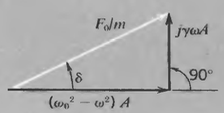
\includegraphics[scale=0.65]{phys232/Ch4-forced-damping-vectors.png} \caption{Graphical representation of \eqref{ch4:eq-forced-with-b-NL}.}	\label{ch4:fig-damping-vectors}
\end{marginfigure}

From the geometry of the triangle:
\begin{align}
	A(\omega_0^2 - \omega^2 ) &= \frac{F_0}{m} \cos\delta \label{ch4:eq-damping-vectors-x} \\
	\gamma\omega A &= \frac{F_0}{m} \sin\delta \label{ch4:eq-damping-vectors-y}
\end{align}

Therefore:%
\footnote{Our expression for $\tan\delta(\omega)$ comes from dividing \eqref{ch4:eq-damping-vectors-y} by \eqref{ch4:eq-damping-vectors-x}. Our result for $A(\omega)$ comes from using the trigonometric identity $\cos^2\theta+\sin^2\theta=1$ after summing the square of the two equations.}%
\begin{equation}
\boxed{
	\begin{split}
		x &= A \cos (\omega t - \delta) \\
		\text{where }
		A(\omega) &= \frac{F_0/m}{[(\omega_0^2 - \omega^2)^2 + (\gamma\omega)^2]^{1/2}} \\
		\tan \delta (\omega) &= \frac{\gamma\omega}{\omega_0^2 - \omega^2}
	\end{split}
}
\label{ch4:eq-soln-b}
\end{equation}

\begin{marginfigure}
	\centering
	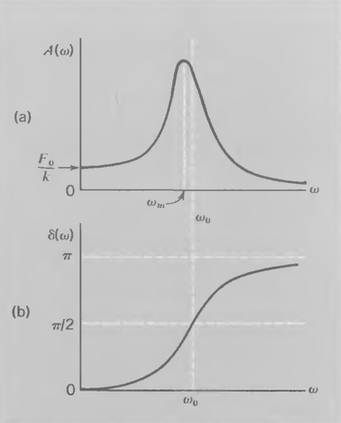
\includegraphics[scale=0.5]{phys232/Ch4-forced-damping-A.png} \caption{(a) Absolute amplitude of forced oscillations (with damping) as a function of $\omega$; (b) phase lag of $x$ with respect to the driving force, as a function of $\omega$.}	\label{ch4:fig-damping-A}
\end{marginfigure}

The results in \eqref{ch4:eq-soln-b} are plotted in Figure~\ref{ch4:fig-damping-A}. Observations:
\begin{itemize}
	\item The curves generally resemble their counterparts in Figure~\ref{ch4:fig-no-damping-A}, where there was no damping.
	\item The phase lag $\delta$ now increases continuously from 0° to 180°. We have $\delta=90$° when $\omega=\omega_0$.
	\item The maximum altitude is actually attained at a frequency $\omega_m$, which is somewhat less than $\omega_0$; in practical applications, this difference is negligible.
	\item $A(\omega)$ and $\delta(\omega)$ are independent of adjustable initial starting conditions.
\end{itemize}

\subsection{Effects of varying the resistive term}
Guiding question: how does the steady state of a damped resonant system change for different values of $Q$, all else being equal?

Recall our definition of $Q$, from \eqref{ch3:eq-Q-def}:
\[ Q = \frac{\omega_0}{\gamma} \so \gamma = \frac{\omega_0}{Q} \]

Substitute our expression for $\gamma$ in terms of $Q$ into \eqref{ch4:eq-soln-b}:
\begin{equation*}
	A(\omega) = \frac{F_0/m}{[(\omega^2 - \omega_0^2)^2 + (\omega_0\omega/Q)^2]^{1/2}}
	\htab
	\tan \delta (\omega) = \frac{\omega\omega_0/Q}{\omega_0^2 - \omega^2}
\end{equation*}

We often graph $A$ and $\delta$ with respect to $\omega/\omega_0$, rather than $\omega$ itself.
\begin{align}
	A&= \frac{F_0}{m}
		\frac{1}{\omega\omega_0 
			\left[(\frac{\omega_0}{\omega} - \frac{\omega}{\omega_0}^2)^2 + \frac{1}{Q^2}
			\right]^{1/2}} \notag \\
	&= \frac{F_0}{m\omega_0^2}
	\frac{\omega_0/\omega}
		{\left[(\frac{\omega_0}{\omega} - \frac{\omega}{\omega_0}^2)^2 + \frac{1}{Q^2}
		\right]^{1/2}} \mathnote{multiplied numerator \& denominator by $\omega_0$ \& moved $\omega$ into the numerator} \notag \\
	&= \frac{F_0}{k}
	\frac{\omega_0/\omega}
		{\left[(\frac{\omega_0}{\omega} - \frac{\omega}{\omega_0}^2)^2 + \frac{1}{Q^2}
		\right]^{1/2}} 	\mathnote{since $k=m\omega^2$}	\label{ch4:eq-damped-A-vs-w/w0}
\intertext{and}
	\tan\delta &= \frac{1/Q}{\frac{\omega_0}{\omega} - \frac{\omega}{\omega_0}}  \mathnote{divided numerator \& denominator by $\omega\omega_0$}	\label{ch4:eq-damped-d-vs-w/w0}
\end{align}

\begin{fullwidth}
\begin{figure}
	\centering
	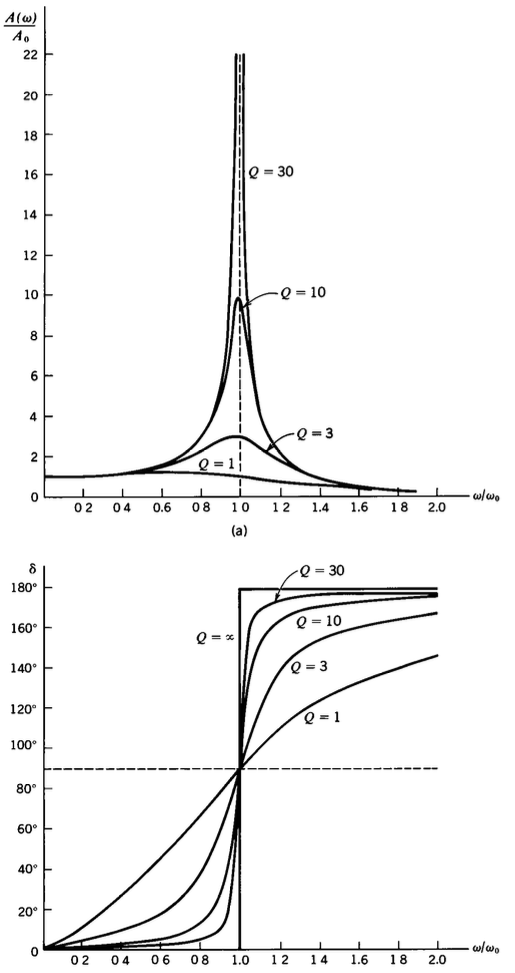
\includegraphics[scale=0.6]{phys232/Ch4-A-delta-vs-Q.png} \caption{(a) Amplitude as a function of $\omega$ for different values of $Q$; (b) phase difference $\delta$ as a function of $\omega$ for different values of $Q$.}	\label{ch4:fig-A-delta-vs-Q}
\end{figure}
\end{fullwidth}

Our results %\eqref{ch4:eq-damped-A-vs-w/w0} and \eqref{ch4:eq-damped-d-vs-w/w0} 
are plotted in Figure~\ref{ch4:fig-A-delta-vs-Q} for different values of $Q$. Observations:
\begin{itemize}
	\item Most of the change in $\delta$ takes place over a band of width $2\omega_0/Q$ centered on $\omega=\omega_0$; i.e. between $\omega=\omega_0(1-1/Q)$ and $\omega=\omega_0(1+1/Q)$.
	\item As $Q\to\infty$, our system behaves like an undamped driven system. $Q\to 0$ represents a heavily damped system.
	\item A maximum amplitude $A_m$ exists for $Q>1/\sqrt{2}$ (i.e. a system that is not ``too damped"); this happens at a frequency $\omega_m < \omega_0$.
\end{itemize}

Searching for the maximum value of $A(\omega)$ in \eqref{ch4:eq-soln-b}, we obtain:
\begin{equation}
\boxed{
	\omega_m = \omega_0 \left( 1-\frac{1}{2Q^2} \right)^{1/2} \andd
	A_m = A_0 \frac{Q}{\left( 1-\frac{1}{4Q^2} \right)^{1/2}} 
}	\label{ch4:eq-damping-Am}
\end{equation}
where $A_0=F_0/k$, i.e. the amplitude obtained for $\omega\to 0$.

\section{Transient State}
Suppose that for $t<0$, our system is at rest at position $x=0$, and that at $t=0$, the driving force is turned on.

\subsection{No damping}
Without damping, the motion of the system is described by \eqref{ch4:eq-no-b}:
\begin{align}
	\mcol{m}\ddot{x} + \kcol{k}x &= F_0 \cos(\omega t) \notag \\
	\Longrightarrow \ddot{x} + \omega_0^2 x &= F_0 \cos(\omega t) 	\label{ch4:eq-no-b-omega2}
\end{align}

Its solution was \eqref{ch4:eq-soln-no-b}:
\[ x(t) = \frac{F_0/m} {\omega_0^2 - \omega^2} \cos(\omega t) \]

This solution is impossible, as it gives $x(0) \neq 0$. 
Assume instead a different solution: 
$$x = x_1 + x_2$$
where $x_1$ is a solution to \eqref{ch4:eq-no-b-omega2}, and $x_2$ is a solution to the equation of free vibration, such that:
\begin{equation*}
	\dder{x_1}{t} + \omega_0^2 x_1 = F_0 \cos(\omega t)  \andd
	\dder{x_2}{t} + \omega_0^2 x_2 = 0
\end{equation*}

Adding the two equations gives:
\[ \dder{(x_1+x_2)}{t} + \omega_0^2(x_1+x_2) = \frac{F_0}{m} \cos(\omega t) \]

This shows that $(x_1+x_2)$ is a more general solution to \eqref{ch4:eq-no-b-omega2} than $x_1$ alone. In addition, $x_2$ gives us two adjustable constants -- amplitude%
\footnote{``B" stands for ``beginning".}
$B$ and initial phase $\beta$.

Let us propose the following solution:
\begin{equation}
	x = \underbrace{B\cos(\omega_0 t + \beta)}_\text{free vibration} + \underbrace{C\cos(\omega t)}_\text{driving force}
	\where
	C = \frac{F_0/m}{\omega_0^2 - \omega^2}
	\label{ch4:eq-transient-no-b-proposed-sol}
\end{equation}

Since $x(0)=0$, \eqref{ch4:eq-transient-no-b-proposed-sol} becomes:
\[ 0 = B\cos\beta + C \]

And since $\dot{x}(0) = 0 = -B\omega_0 \cos(\omega_0 t + \beta) - \omega C \sin(\omega t)$:
\[ 0 = -B\omega_0 \sin\beta \]

If we take $\beta=0$, we get $B=-C$. Therefore:
\begin{equation}
\boxed{
	x = C(\cos(\omega t) - \cos(\omega_0 t))
	\where
	C = \frac{F_0/m}{\omega_0^2 - \omega^2}
}
\label{ch4:eq-transient-no-b-sol}
\end{equation}

Observations about \eqref{ch4:eq-transient-no-b-sol}:
\begin{itemize}
	\item This is an example of beats.
	\item Without damping, these beats would continue on indefinitely, and no steady state would ever be reached.
\end{itemize}

The conditions just after $t=0$ now make sense; if $\omega t, \omega_0 t \ll 1$, we have%
\footnote{By the small angle approximation in \eqref{ch1:eq-small-angle-cos}: $\cos\theta \approx 1-\theta^2/2$}:
\begin{equation*}
	\cos(\omega t) \approx 1 - \frac{\omega^2 t^2}{2} \andd \cos(\omega_0 t) \approx 1 - \frac{\omega_0^2 t^2}{2}
\end{equation*}
\begin{equation*}
	\Longrightarrow
	x \approx \frac{F_0/m}{\omega_0^2 - \omega^2} \frac{(\omega_0^2 - \omega^2)t^2}{2} 
	\approx \frac{1}{2} \frac{F_0}{m} t^2
\end{equation*}

This tells us that before the restoring forces come into play, we have displacement $x$ in the same direction as the driving force, with acceleration $F_0/m$.

\subsection{With damping}

Our solution is:
\begin{equation}
\boxed{
	\begin{split}
		&x = \underbrace{Be^{-\gamma t/2} \cos(\omega_1 t + \beta)}_\text{transient} + \underbrace{A\cos(\omega t - \delta)}_\text{driving force}
		\\
		&\text{where }
		\omega_1 = \left(\omega_0^2 - \frac{\gamma^2}{4} \right)^{1/2}
	\end{split}
}	\label{ch4:eq-transient-with-b-sol}
\end{equation}

Note that the transient part of \eqref{ch4:eq-transient-with-b-sol} accounts for our adjustable initial conditions $A, \delta$, given by \eqref{ch4:eq-soln-b}.



\section{Power}
Power required to keep a driven oscillator going at the same amplitude:
\[ P = \frac{dW}{dt} = F\frac{dx}{dt} = Fv \]